\begin{figure}
	\centering
	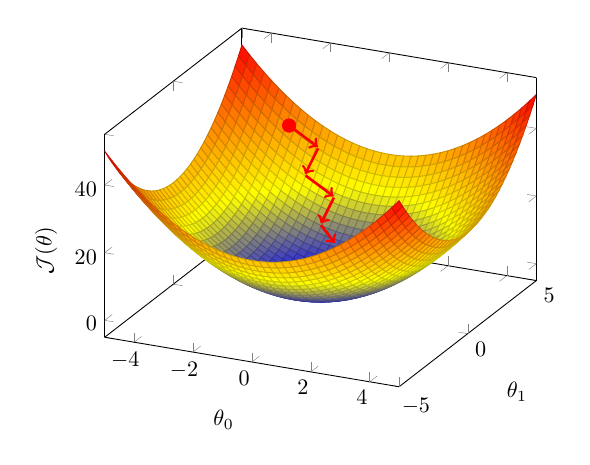
\begin{tikzpicture}[
		scale=0.80,
		arr/.style={
			shorten >=0.15mm,shorten <=0.15mm,->,red,very thick
		}
	]
		\begin{axis}[
			xlabel=$\theta_0$,
			ylabel=$\theta_1$,
			zlabel=$\mathcal{J}(\bm{\theta})$
		]
	
			\addplot3[
				surf,
				samples=41
			] {x^2+y^2};

			\draw[draw=red,fill=red] (axis cs:-2,2,40) circle (3pt);
			\draw[arr] (axis cs:-2,2,40) -- (axis cs:-1,2,35);
			\draw[arr] (axis cs:-1,2,35) -- (axis cs:-1,1,30);
			\draw[arr] (axis cs:-1,1,30) -- (axis cs:0,1,25);
			\draw[arr] (axis cs:0,1,25) -- (axis cs:0,0,20);
			\draw[arr] (axis cs:0,0,20) -- (axis cs:0.5,0,15);
		\end{axis}
	\end{tikzpicture}
\end{figure}